%-------------------------------------------------------------------------------------------------%
\documentclass[12pt]{article}
%-------------------------------------------------------------------------------------------------%
\usepackage[spanish]{babel}
\usepackage[margin=1in]{geometry}
\usepackage[hidelinks]{hyperref}
\usepackage{amssymb,amsmath,amsthm,amsfonts}
\usepackage{enumerate}
\usepackage{graphicx}
\usepackage{datetime}
\usepackage{parskip}
\usepackage{apacite}
\usepackage{lipsum}
\usepackage{color}
\usepackage{float}
\usepackage{cancel}
\usepackage[framed,numbered,autolinebreaks,useliterate]{mcode}
%-------------------------------------------------------------------------------------------------%
\newenvironment{solution}{\begin{proof}[Solución]}{\end{proof}}
\renewcommand{\qedsymbol}{\rule{0.7em}{0.7em}}
\newtheorem{proposition}{Proposición}
\newtheorem{observation}{Observación}
\newtheorem{afirmation}{Afirmación}
\newtheorem{definition}{Definición}
\newtheorem{corollary}{Corolario}
\newtheorem{exercise}{Ejercicio}
\newtheorem{theorem}{Teorema}
\newtheorem{example}{Ejemplo}
\newtheorem{lemma}{Lema}
\graphicspath{{Img/}}
\decimalpoint
%-------------------------------------------------------------------------------------------------%
\title{Tarea 5 - Optimización No Lineal}
\author{Camara Medina Cynthia Lilian \\[0.5cm]
Alanis González Edzon Omar}
\date{\today}
%-------------------------------------------------------------------------------------------------%
\makeatletter
\let\thetitle\@title
\let\theauthor\@author
\let\thedate\@date
\makeatother
%-------------------------------------------------------------------------------------------------%
\begin{document}
%-------------------------------------------------------------------------------------------------%
\begin{titlepage}
\centering

\includegraphics[width=0.9\linewidth]{../logo.png}\\[2.0 cm]
\textsc{\LARGE Escuela Superior de Física y Matemáticas}\\[1.2 cm]
\textsc{\Large Instituto Politécnico Nacional}\\[2.5 cm]
\rule{\linewidth}{0.2 mm} \\[0.4 cm]
{\huge \bfseries \thetitle}\\
\rule{\linewidth}{0.2 mm} \\[2.5 cm]
\textsc{\large \theauthor}
\vfill
{\large \thedate}
\end{titlepage}
%-------------------------------------------------------------------------------------------------%

\section*{Investigación}

\begin{enumerate}
    \item Dada una matriz simétrica, explique cómo se puede determinar si esta es o no definida positiva.
    
    Una matriz simétrica real $A$ es:
    \begin{itemize}
        \item Definida \textbf{positiva}: Si $X A \; \; X^{t} \geq 0$ para cualquier vector $X=(x_1,\dots,x_n) \in Mat_{1\times n}(\mathbb{R})$
        \item Definida \textbf{negativa}: Si $X A \; \; X^{t} \leq 0$ para cualquier vector $X=(x_1,\dots,x_n) \in Mat_{1\times n}(\mathbb{R})$
        
        Por el criterio de Sylvester
        \begin{theorem}[Criterio de Sylvester]
            Sea $A \in Mat_{n\times n}(\mathbb{R})$ una matriz simétrica real, y
            \[\Delta_j = det \begin{pmatrix}
                a_{11} & \cdots & a_{1j} \\
                \vdots & & \vdots \\
                a_{j1} & \cdots & a_{jj}
            \end{pmatrix}\] entonces
            \begin{enumerate}[I.]
                \item Si $\Delta_j >0$ para $j=1,\dots,n$, entonces $A$ es definida \textbf{positiva}.
                \item Si $(-1)^j\Delta_j <0$ para $j=1,\dots,n$, entonces $A$ es definida \textbf{negativa}.
            \end{enumerate}
        \end{theorem}
    \end{itemize}
    \item Investigue la definición de una función convexa de varias variables.
    
    Una función $f(x_1,\dots,x_n)$ es convexa si cumple las siguientes dos condiciones:

    \begin{itemize}
        \item El dominio de la función $dom (f)$ es un conjunto convexo en $R^n$
        \item Para todo $b_1 = (b_{11}, \dots, b_{1n}), b_2 = (b_{21},\dots,b_{2n})$ puntos en $dom(f)$ y $\alpha \in [0,1]$ se cumple que
        \[f(\alpha b_1 + (1-\alpha)b_2) \leq \alpha f(b_1)+(1-\alpha)f(b_2)\]
    \end{itemize}
    \item Enuncie e ilustre dos propiedades de las funciones convexas en $\mathbb{R}^n$
    \begin{itemize}
        \item Si una función $f:\mathbb{R}^n \rightarrow \mathbb{R}^n$ es convexa y derivable, la minimización de la función es equivalente a la solución de $\nabla f(x) =0$
        \item Una función  $f:\mathbb{R}^n \rightarrow \mathbb{R}^n$ de la clase $C^2$ es convexa si y solo si su matriz Hessiana $\nabla^2f(x)$ es semi definida positiva $\forall x \in \mathbb{R}^n$  
    \end{itemize}
\end{enumerate}

\newpage

\section*{Ejercicios}

\textbf{Condiciones de optimalidad para varias variables}

\begin{enumerate}
    \item Hallar y clasificar todos los puntos estacionarios del siguiente problema:
    \[f(x_1,x_2) = 2x_1^2+4x_1x_2^3-10x_1x_2+x_2^2\]
    \begin{figure}[H]
        \centering
        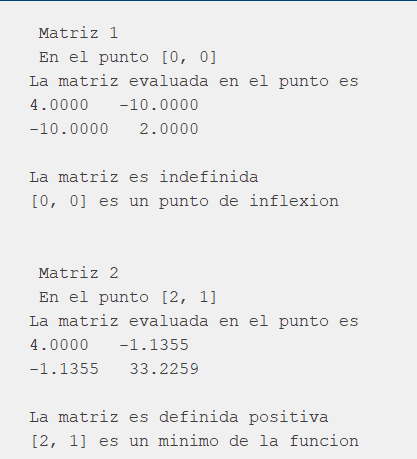
\includegraphics[width = 0.4\textwidth]{1-1.png}
        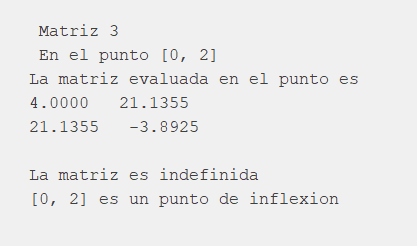
\includegraphics[width = 0.4\textwidth]{1-2.png}
    \end{figure}
    \begin{figure}[H]
        \centering
        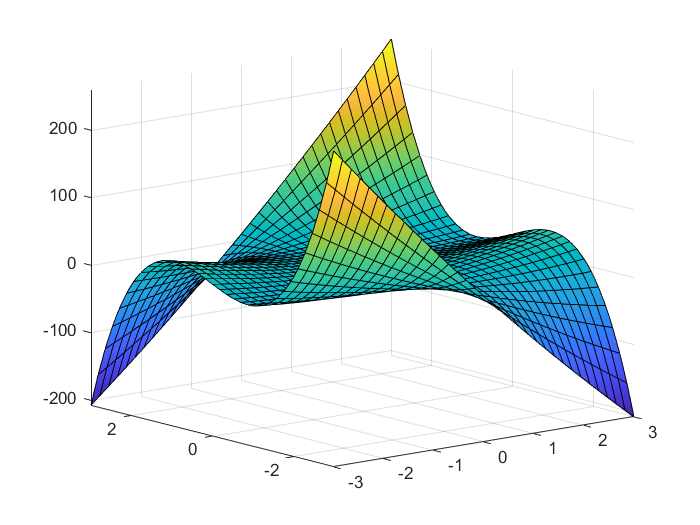
\includegraphics[width = 0.4\textwidth]{1-3.png}
        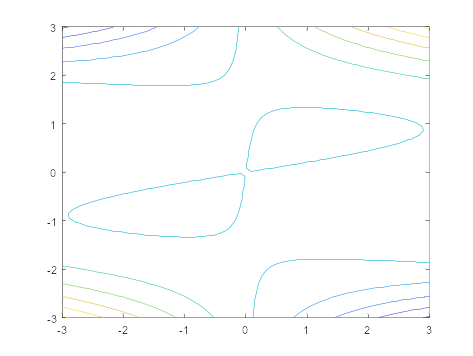
\includegraphics[width = 0.4\textwidth]{1-4.png}
    \end{figure}
    \newpage
    \item Hallar y clasificar todos los puntos estacionarios del siguiente problema:
    \[f(x_1,x_2) = (x_1-2)^2+(x_1-2x_2^2)^2\]
    \begin{figure}[H]
        \centering
        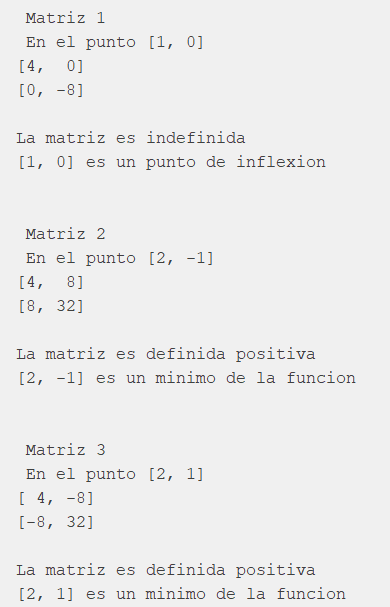
\includegraphics[width = 0.4\textwidth]{2-1.png}
    \end{figure}
    \begin{figure}[H]
        \centering
        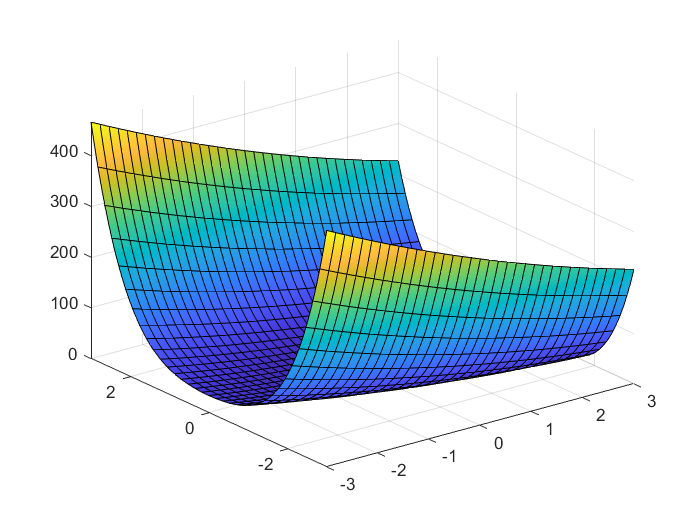
\includegraphics[width = 0.4\textwidth]{2-2.png}
        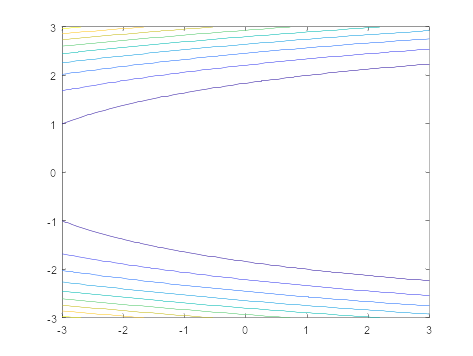
\includegraphics[width = 0.4\textwidth]{2-3.png}
    \end{figure}
    \newpage
    \item Hallar y clasificar todos los puntos estacionarios del siguiente problema:
    \[f(x_1,x_2) = 25x_1^2-12x_1^4-6x_1x_2+25x_2-24x_1^2x_2^2-12x_2^2\]
    \begin{figure}[H]
        \centering
        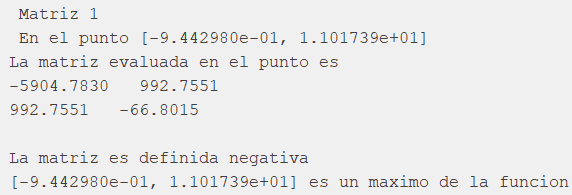
\includegraphics[width = 0.6\textwidth]{3-1.png}
        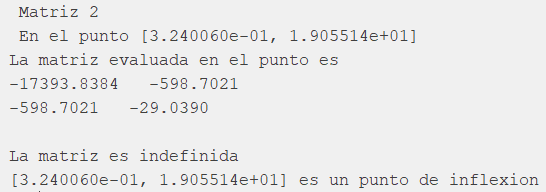
\includegraphics[width = 0.6\textwidth]{3-2.png}
        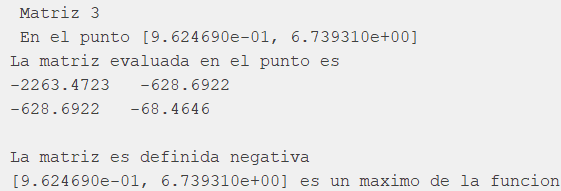
\includegraphics[width = 0.6\textwidth]{3-3.png}
    \end{figure}
    \begin{figure}[H]
        \centering
        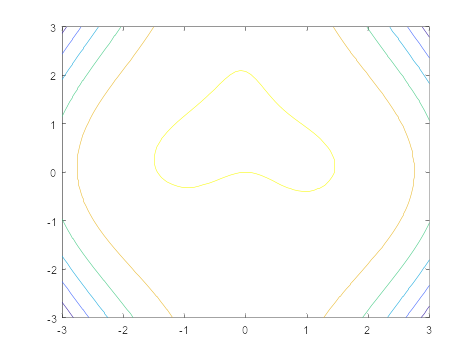
\includegraphics[width = 0.4\textwidth]{3-4.png}
        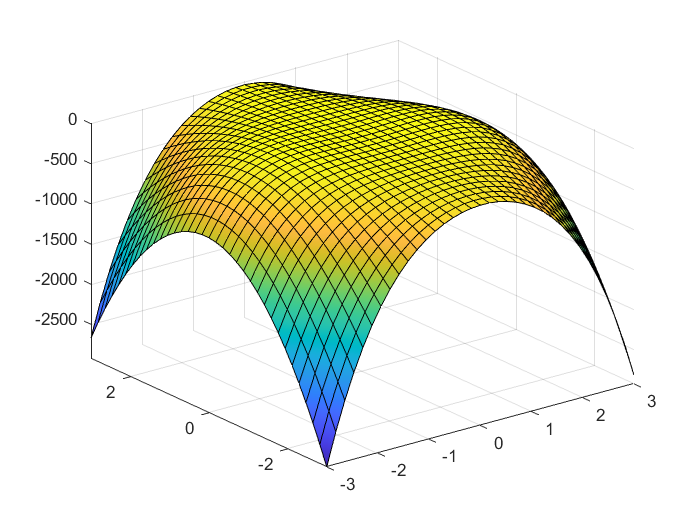
\includegraphics[width = 0.4\textwidth]{3-5.png}
    \end{figure}
\end{enumerate}

\newpage

\section*{Programación}

\begin{lstlisting}
    %%% MATRIZ HESSIANA %%%

    clear;
    clc;
    
    f = input('\n Ingresar la funcion:\n');
    %Funcion anonima con indices
    
    v = input('\n Ingresa el punto x para evaluar:\n');
    %Ingresar como vector
    
    
    h = 1E-5;
    n = length(v); %Tamano del vector de valores iniciales
    a = h.*eye(n); %Matriz identidad  

    Hess=ones(n);

    for k= 1:n %Sera el que controle respecto a que variable se esta derivando
        for j=1:n
            Hess(j,k) = (1/(h^2))*(f(v+a(k,:)+a(j,:))- f(v+a(k,:))- f(v+a(j,:))+f(v));
            Entrada=round(Hess,3,"significant");
        end % for j
    end %for k

    fprintf('\n Matriz Hessiana en el punto dado es \n'); %Hessiana
    disp(Entrada);
\end{lstlisting}

\section*{Bibliografía}

\begin{itemize}
    \item \url{https://ocw.ehu.eus/pluginfile.php/42576/mod_page/content/1/tema4_7.pdf}
    \item \url{http://www.ifp.illinois.edu/~angelia/L3_convfunc.pdf}
    \item \url{https://wiki.math.ntnu.no/_media/tma4180/2016v/note2.pdf}
\end{itemize}



%-------------------------------------------------------------------------------------------------%
\end{document}
%-------------------------------------------------------------------------------------------------%